\section{Overview} \label{sec:overview}

\begin{figure*}[t!] 
     \centering 
     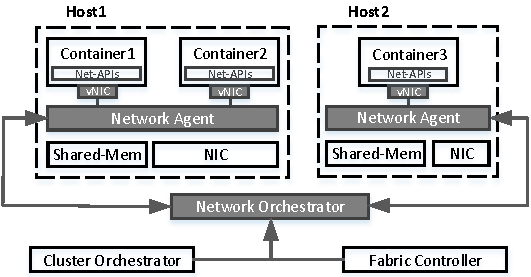
\includegraphics[width=7in]{figures/system-arch.pdf} 
    \caption{\label{fig:sysarch} The overall system architecture of existing overlay network and \sysname. Gray boxes are building blocks of~\sysname.}
\end{figure*} 

In this section, we discuss the overall architecture of \sysname, and discuss the
key insights that enable \sysname to achieve a high network performance without
sacrificing portability of containers.

\subsection{High network performance without sacrificing portability}

Container deployments opt for overlay-based networking since it is most
portable: a container does not have to worry about where the other endpoint is.
For example, in Figure~\ref{fig:sysarch}(a), Container~1 and Container~3 cannot
distinguish whether Container~2 is on Host~1 or Host~2, as long as Container~2
keeps its overlay IP address (2.2.2.2) and the overlay routers know how to
route packets to this IP. 

Existing overlay-based container networks sacrifice performance for good
portability, because traffic needs to go through a deep software stack, as shown
in Figure~\ref{fig:sysarch}(a).  The key to achieve high performance and low
overhead overlay network for containers is to avoid, in the data-plane, any
performance bottlenecks such as bridges, software routers and host OS kernel.
Given that containers are essentially processes, the communication channels
provided by host-based IPC and hardware offloaded network transports (RDMA) give
us numerous options to build a better container network. For instance,
containers within a single host, like Container~1 and Container~2 in
Figure~\ref{fig:sysarch}(a), can communicate via a shared-memory channel, and
overlay routers in different hosts can talk via RDMA (or DPDK) to
bypass the performance bottlenecks. Note that communication paradigms like
shared-memory and RDMA partially sacrifice the isolation of containers. However,
since in most cases containers that communicate with each other are part of the
same larger, distributed application deployed by a single tenant. Therefore, we
believe that that trading off a little isolation for a large boost in
performance is acceptable.  We will discuss security implications of our design
in more detail later in the paper.

%% Even today, containers isolation is considered
%% inadequate for untrusted workloads~\cite{containers-blackhat,containers-rhel,containers-rhel}.

Generally, one container should decide how to communicate with another according
to the latter's location, using the optimal transport for high networking
performance.  There are two issues to realize this key idea: (1) How to discover
the real-time locations of containers; (2) How to enable containers to use
different mechanisms to communicate with different peers.

One way is to solve these two issues is to depend on containerized applications
themselves: the applications can discover and exchange location information and
agree on a communication mechanism to use. This method requires applications to
do extra work (and the code can become quite complicated, as the programmer
deals with different communication methods), and hence is undesirable. 

Instead, we take an alternative approach: using a (conceptually) centralized
orchestrator to decide how containers should communicate, and keeping the
container locations and the actual communication mechanisms transparent to
containerized applications. Our key insight is that since currently most of the
container clusters are managed by a centralized cluster orchestrator (e.g., Mesos,
Kubernetes, and Docker Swarm)\footnote{They can easily be deployed on private
bare-metal clusters or cloud VM clusters without any special supports from cloud
providers.}, the information about the location of the other endpoints can be
easily obtained by querying the orchestrator. By leveraging this information, we
can choose the right communication paradigm for the specific scenario.
Furthermore, all of the complexity of communication mechanism selection and
execution can be hidden from the application by bundling it into a customized
network library supporting standard network APIs.  Next, we sketch the
architecture of our solution.

\subsection{The architecture of FreeFlow}

Figure~\ref{fig:sysarch}(a) shows the architecture of existing overlay
networking solutions for containers. Each container has a virtual NIC that is
attached to the overlay router of the host via software bridge. Different
overlay routers exchange routing information and build routing tables via
standard routing protocols, such as BGP. The fabric built by virtual NICs,
bridges, overlay routers, physical NICs and the host network is the
actual data-plane for packets traversing the overlay from container to another
one. Inside each container, applications use standard network APIs to access the
network. The API calls are implemented in network libraries, such as
\texttt{glibc} for Socket API, and \texttt{libibverbs} for RDMA Verbs API.

\sysname reuses many control-plane features like IP allocation and routing
implemented by existing solutions such as {\em Weave}.  However, \sysname
modifies multiple existing modules in the networking stack to achieve a smarter
and more efficient data-plane.

Figure~\ref{fig:sysarch}(b) shows the overall architecture of \sysname.  The
gray boxes in Figure~\ref{fig:sysarch}(b) represent the three key building
blocks of \sysname: customized network library, customized overlay router and
customized orchestrator.

\sysname's network library is the core component which decides which
communication paradigm to use. It supports standard network programming APIs,
e.g. Socket for TCP/IP, MPI and Verbs for RDMA, etc. It queries the network
orchestrator for the location of the container it wishes to communicate with.
Whenever possible, it uses shared memory to communicate with the other
container, bypassing overlay router.  \sysname's overlay routers are based on
existing overlay routers. We add two new features: (1) the traffic between
routers and its local containers goes through shared-memory instead of software
bridge; and (2) the traffic between different routers is delivered via kernel
bypassing techniques, e.g. RDMA or DPDK, if the hardware on the hosts is
capable.  Network orchestrator keeps track of the realtime locations of each
container in the cluster. Our solution extends existing network orchestration
solutions, and allows \sysname's network library to query for the physical
deployment location of each container. 

The architecture enables the possibility to make traffic among containers flow
through an efficient data-plane: shared-memory for intra-host cases and
shared-memory plus kernel bypassing networking for inter-host cases.

However, we have two challenges to achieve \sysname's simple vision.  First, the
network library of \sysname should naturally support multiple standard network
APIs for transparency and backward compatibility. Second, for inter-host cases,
overlay routers should connect the shared-memory channel with local containers
and the kernel bypassing channel between physical NICs to avoid overhead caused
by memory copying. In next section, we discuss how \sysname addresses these
challenges.
